\subsection{Chebyshev Polynomials(Optional)}

\frame{
We now turn our attention to polynomial interpolation for $f(x)$ over $[-1,1]$ based on the nodes $-1 \le x_0 < x_1 < \cdots < x_N \le 1$. Both the Lagrange and Newton polynomials satisfy
\begin{equation*}
f (x) = P_N (x) + E_N (x)
\end{equation*} 
where 
\begin{equation*}
E_N (x) = Q(x) \frac{f^{(N+1)}(c)}{(N + 1)!}
\end{equation*} 
and $Q(x)$ is the polynomial of degree $N + 1$: 
\begin{equation*}
Q(x) = (x - x_0)(x - x_1) \cdots (x - x_N ).
\end{equation*} 
}

\frame{
Using the relationship 
\begin{equation*}
\left| E_N (x) \right| \le \left| Q(x) \right| \frac{\max_{-1 \le x \le 1} \left\{ \left| f ^{N+1)} (x) \right| \right\} }{ (N + 1)!}
\end{equation*} 
our task is to follow Chebyshev's derivation on how to select the set of nodes $\{x_k\}^N_{k=o}$ that minimizes $max_{-1 \le x \le 1} \{ | Q(x) |\} $. 
}


\frame{
This leads us to a discussion of Chebyshev polynomials and some of their properties. 
\begin{center}
$\Downarrow$
\end{center}
To begin, the first eight Chebyshev polynomials are listed in the following table. 
\begin{figure}
\begin{center}
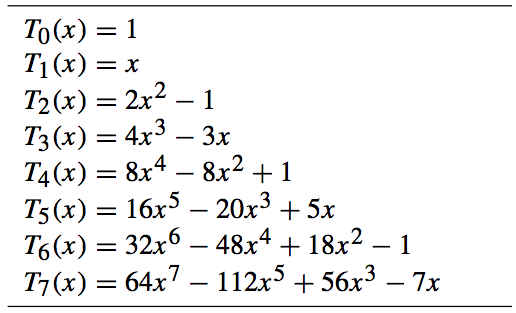
\includegraphics[width=60mm]{chap-3/tab_4-11.png}
\end{center}
\end{figure} 
}

\frame{
\frametitle{Properties of Chebyshev Polynomials}
\begin{block}{Property 1. Recurrence Relation} 
Chebyshev polynomials can be generated in the following way. 
Set $T_0(x) = 1$ $T_1 (x) = x$ and use the recurrence relation 
\begin{equation*}
T_k (x) = 2x T_{k-1}(x) - T_{k-2}(x)  \ \ \  for \ \ k = 2, 3, \ldots
\end{equation*} 
\end{block}
Property 1 is often used as the definition for higher-order Chebyshev polynomials. 
Let us show that $T_3(x) = 2xT_2(x) - T_1(x)$. 
\begin{center}
$\Downarrow$
\end{center}
Using the expressions for $T_1(x)$ and $T_2(x)$ in Table 3.11, we obtain 
\begin{equation*}
2x T_2 (x) - T_1(x) = 2x \left( 2x^2 -1 \right) - x = 4 x^3 - 3 x - T_3(x) 
\end{equation*} 
}

\frame{
\begin{block}{Property 2. Leading Coefficient} 
The coefficient of $x^N$ in $T_N(x)$ is $2^{N-1}$ when $N \ge 1$. 
\end{block}
Property 2 is proved by observing that the recurrence relation doubles the leading coefficient of $T_{N-l}(x)$ to get the leading coefficient of $T_N(x)$, 

\begin{block}{Property 3. Symmetry} 
When $N = 2M$, $T_{2M}(x)$ is an even function, that is,
\begin{equation*}
T_{2M}(-x) = T_{2M}(x).
\end{equation*} 
When $N = 2M + 1$, $T_{2M+1}(x)$ is an odd function, that is,
\begin{equation*}
T_{2M+1}(-x) = -T_{2M+1}(x).
\end{equation*} 
\end{block}
Property 3 is established by showing that $T_{2M} (x)$ involves only even powers of $x$ and $T_{2M+1}(x)$ involves only odd powers of $x$.
%The details are left for the reader. 
}

\frame{
\begin{block}{Property 4. Trigonometric Representation on $[-1, 1]$ }
\begin{equation*}
T_N (x) = \cos(N \arccos(x))    \ \ \ for  \ \ -1 \le x \le 1.
\end{equation*} 
\end{block}
The proof of property 4 uses the trigonometric identity 
\begin{equation*}
cos(k\theta) = cos(2\theta) cos((k - 2)\theta) - sin(2\theta) sin((k - 2)\theta).
\end{equation*} 
Substitute $\cos(2\theta) = 2 \cos^2 (\theta) - 1$ and $\sin(2\theta) = 2 \sin(\theta) \cos(\theta)$ and get
\begin{equation*}
cos(k\theta) = 2 cos(\theta)(cos(\theta) cos((k - 2)\theta) - sin(\theta) sin((k - 2)\theta)) - cos((k - 2)\theta),
\end{equation*} 
which is simplified as 
\begin{equation*}
cos(k\theta) = 2 cos(\theta) cos((k - 1)\theta) - cos((k - 2)\theta).
\end{equation*} 
Finally, substitute $\theta = arccos(x)$ and obtain 
\begin{equation*}
2x cos((k - 1) arccos(x)) - cos((k - 2) arccos(x)) = cos(k arccos(x)) 
\end{equation*} 
for $-1 \le x \le 1$.
}

\frame{
\begin{block}{Property 5. Distinct Zeros in $[-1,1]$} 
$T_N(x)$ has $N$ distinct zeros $x_k$ that lie in the interval $[-1,1]$ (see Figure 3.15):
\begin{equation*}
x_k = \cos \left( \frac{(2k+1) \pi }{2N}\right) \ \ \ for \ \ k = 0, 1, 2, \ldots, N-1
\end{equation*} 
These values are called the {\Large Chebyshev abscissas (nodes)}.
\end{block}
\begin{figure}
\begin{center}
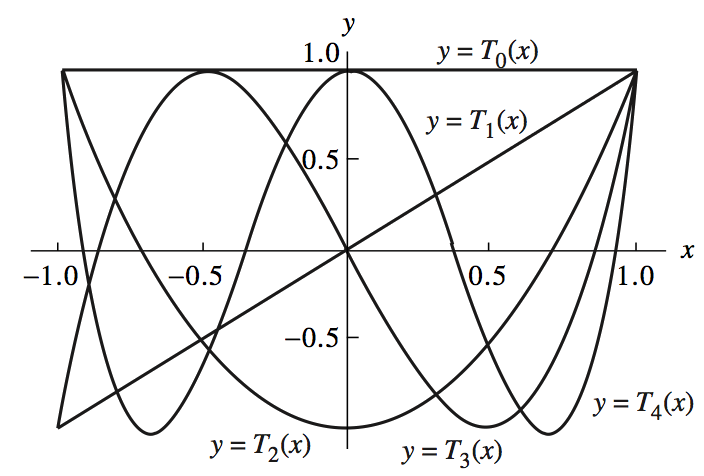
\includegraphics[width=60mm]{chap-3/fig_4-15.png}
\end{center}
\end{figure}
}

\frame{
\begin{block}{Property 6. Extreme Values }
\begin{equation*}
\left| T_N (x) \right| \le 1 \ \ \ for \ \ -l \le x \le 1
\end{equation*}
\end{block}
The first two Chebyshev polynomials are $T_0 (x) = cos(0 arccos(x)) = 1$ and $T_1(x) = cos(1 arccos(x)) = x$. 
Now assume that $T_k(x) = cos(k arccos(x))$ for $k = 2,3, ... ,N-1$. 
Formula (3.79) is used with (3.85) to establish the general case: 
\begin{equation*}
\begin{array}{l c l}
T_N (x) & = & 2x T_{N-1} (x) - T_{N-2}(x) \\
& = &  2x \cos((N - 1) \arccos (x) ) - \cos((N - 2) \arccos(x)) \\
& = &  \cos(N \arccos(x)) \ \ \ for \ \ -1 \le x \le 1.
\end{array}
\end{equation*} 
Properties 5 and 6 are consequences of property 4. 
}

\frame{
\frametitle{Minimax}
\framesubtitle{极小极大}
\begin{itemize}
\item The Russian mathematician Chebyshev studied how to minimize the upper bound for $|E_N(x)|$.
\item One upper bound can be formed by taking the product of the maximum value of $|Q(x)|$ over all $x$ in $[-1,1]$ and the maximum value $|f^{(N+1)} (x) \slash (N + 1)!|$ over all $x$ in $[-1,1]$. 
\item To minimize the factor $max\{ |Q(x)| \}$, Chebyshev discovered that $x_0$, $x_1$, $\ldots$, $x_N$ should be chosen so that $Q(x) = (1 \slash 2^N) T_{N+1}(x)$. 
\end{itemize}
}

\frame{
\begin{block}{Theorem 3.7.} 
Assume that $N$ is fixed. 
Among all possible choices for $Q(x)$, and thus among all possible choices for the distinct nodes $\left\{ x_k \right\}^N_{k=0}$ in $[-1, 1]$,
the polynomial $T (x) = T_{N+1}(x) \slash 2^N$ is the unique choice that has the property
\begin{equation*}
\max_{-1 \le x \le 1} \left\{ \left| T(x) \right| \right\} \le \max_{-1 \le x \le 1} \left\{ \left| Q(x) \right| \right\}
\end{equation*}
Moreover 
\begin{equation*}
\max_{-1 \le x \le 1} \left\{ \left| T(x) \right| \right\} = \frac{1}{2^N}
\end{equation*}
\end{block}
}

\frame{
\frametitle{Proof of Theorem 3.7.}
Let $\prod^{N+1}$ denote the set of all monic polynomials of degree $N+1$. 
Suppose $P_{N+1} \in \prod^{N+1} $ and
\begin{equation*}
\max_{x \in [-1,1]} \left| P_{N+1} (x) \right| \le \frac{1}{2^N} = \max_{x \in [-1,1]}  \left| T (x) \right|
\end{equation*}
Let $Q = T - P_{N+1}$.

Since $|T(x)|$ and $P_{N+1}(x)$ are both monic polynomials of degree $N+1$,
$Q(x)$ is a polynomial of degree at most $N$.
Moreover, at the extreme points $\bar{x}_k'$ of $T(x)$,
\begin{equation*}
Q(\bar{x}_k') = T(\bar{x}_k') - P_{N+1}(\bar{x}_k') = \frac{(-1)^k}{2^N} - P(\bar{x}_k')
\end{equation*} 
}

\frame{
Since
\begin{equation*}
\left| P(\bar{x}_k') \right| \le  \frac{1}{2^N} \ \ \ for \ \ each \ \ k = 0, 1, 2, \ldots, N+1
\end{equation*}
we have $Q(\bar{x}_k') \le 0$ when $k$ is odd and $Q(\bar{x}_k') \ge 0$ when $k$ is even.

Since $Q$ is continuous, the intermediate value throrem implies that the polynomial $Q(x)$ has at least one zero between $\bar{x}'_j$ and $\bar{x}'_{j+1}$ for each $j=0,1,\ldots,N$.
Thus $Q$ has at least $N+1$ zeros in intervl $[-1,1]$.
But the degree of $Q(x)$ is less than $N+1$, so $Q \equiv 0$.
This implies that $P_{N+1} \equiv T$
%\begin{figure}
%\begin{center}
%\includegraphics[width=110mm]{fig/ch-3/theorem_3-7_proof-2.png}
%\end{center}
%\end{figure} 
}

\frame{
The consequence of this result can be stated by saying that for Lagrange interpolation $f (x) = P_N (x) + E_N (x)$ on $[-1, 1]$, 
the minimum value of the error bound
\begin{equation*}
\left( \max{ |Q(x)| } \right) \left( \max \left\{ \left| f^{(N+1)}(x) \slash (N + 1)! \right| \right\} \right)
\end{equation*}
is achieved when the nodes $\{ x_k \}$ are the Chebyshev abscissas of $T_{N+1}(x)$.
As an illustration,
we look at the Lagrange coefficient polynomials that are used in forming $P_3(x)$. 
First we use equally spaced nodes and then the Chebyshev nodes. 
Recall that the Lagrange polynomial of degree $N = 3$ has the form
\begin{equation*}
P_3(x) = f (x_0)L_{3,0}(x) + f (x_1)L_{3,1}(x) + f (x_2)L_{3,2}(x) + f (x_3)L_{3,3}(x).
\end{equation*}
}

\frame{
\frametitle{Equally Spaced Nodes}
\begin{itemize}
\item If $f (x)$ is approximated by a polynomial of degree at most $N = 3$ on $[-1, 1]$, the equally spaced nodes $x_0 = -1$, $x_1 = -1 \slash 3$, $x_2 = 1 \slash 3$, and $x_3 = 1$ are easy to use for calculations. 
\item Substitution of these values into formula (3.27) of Section 3.3 and simplifying will produce the coefficient polynomials $L_{3,k}(x)$ in Table 3.12. 
\end{itemize}
\begin{figure}
\begin{center}
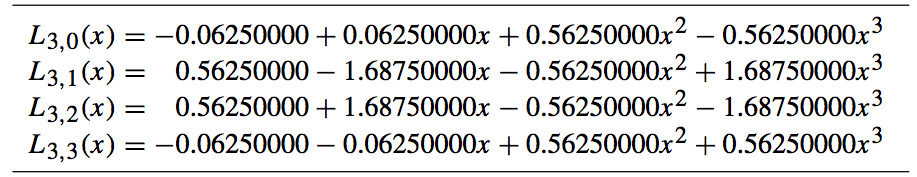
\includegraphics[width=80mm]{chap-3/tab_4-12.png}
\end{center}
\end{figure} 
}

\frame{
\frametitle{Chebyshev Nodes}
When $f(x)$ is to be approximated by a polynomial of degree at most $N = 3$, using the Chebyshev nodes $x_0 = \cos( 7 \pi \slash8)$, $x_1 = \cos(5\pi \slash 8)$, $x_2 = \cos(3\pi \slash 8)$, and $x_3 = \cos(\pi \slash 8)$, the coefficient polynomials are tedious to find (but this can be done by a computer). 
The results after simplification are shown in Table 3.13.
\begin{figure}
\begin{center}
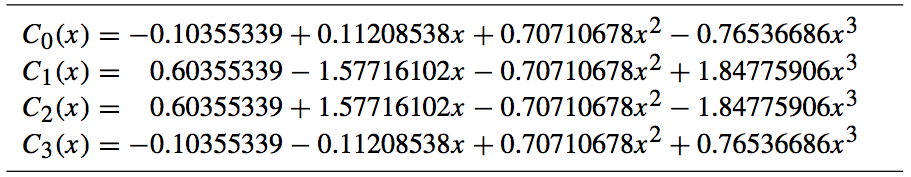
\includegraphics[width=100mm]{chap-3/tab_4-13.png}
\end{center}
\end{figure} 
}

\frame{
\frametitle{Example 3.14.} 
Compare the Lagrange polynomials of degree $N = 3$ for $f (x) = e^x$ that are obtained by using the coefficient polynomials in Tables 3.12 and 3.13, respectively.
Using equally spaced nodes, we get the polynomial
\begin{equation*}
 P(x) = 0.99519577 + 0.99904923 x + 0.54788486 x^2 + 0.17615196 x^3
\end{equation*}

This is obtained by finding the function values
\begin{equation*}
\begin{array}{l l}
f (x_0) = e^{(-1)}  = 0.36787944,  & f (x_1) = e^{(-1 \slash 3)} = 0.71653131, \\
f (x_2) = e^{(1 \slash 3)} = 1.39561243,  & f (x_3) = e^{(1)} = 2.71828183,
\end{array}
\end{equation*}
and using the coefficient polynomials $L_{3,k} (x)$ in Table 3.12, and forming the linear combination
\begin{equation*}
\begin{array}{l c l}
P(x) & = & 0.36787944L_{3,0}(x) + 0.71653131L_{3,1}(x) + 1.39561243L_{3,2}(x) \\
& & + 2.71828183L_{3,3}(x).
\end{array}
\end{equation*}
}

\frame{
Similarly, when the Chebyshev nodes are used, we obtain
\begin{equation*}
V(x) = 0.99461532 + 0.99893323x + 0.54290072x^2 + 0.17517569x^3.
\end{equation*}
Notice that the coefficients are different from those of $P(x)$. 
This is a consequence of using different nodes and function values:
\begin{equation*}
\begin{array}{l c l c l} 
f (x_0) & = & e^{-0.92387953} & = & 0.39697597, \\
f (x_1) & = & e^{-0.38268343} & = & 0.68202877, \\
f (x_2) & = & e^{0.38268343}   & = & 1.46621380, \\
f (x_3) & = & e^{0.92387953}   & = & 2.51904417.
\end{array}
\end{equation*}
Then the alternative set of coefficient polynomials $C_k (x)$ in Table 4.13 is used to form the linear combination
\begin{equation*}
V(x)= 0.39697597 C_0(x) + 0.68202877 C_1(x) + 1.46621380 C_2(x) + 2.51904417 C_3(x).
\end{equation*}
}

\frame{
For a comparison of the accuracy of $P(x)$ and $V(x)$, the error functions are graphed in the following figures. 
The maximum error $\left| e^x - P(x) \right|$ occurs at $x = 0.75490129$, and
\begin{equation*}
\left| e^x - P(x) \right| \le  0.00998481 \ \ \ for \ \ -1 \le x \le 1.
\end{equation*}
The maximum error $\left| e^x - V(x) \right|$ occurs at $x = 1$, and we get
\begin{equation*}
\left| e^x - P(x) \right| \le  0.00665687 \ \ \ for \ \ -1 \le x \le 1.
\end{equation*}
Notice that the maximum error in $V(x)$ is about two-thirds the maximum error in $P(x)$.
Also, the error is spread out more evenly over the interval.
\begin{columns}
\begin{column}{0.5\textwidth}
\begin{figure}
\begin{center}
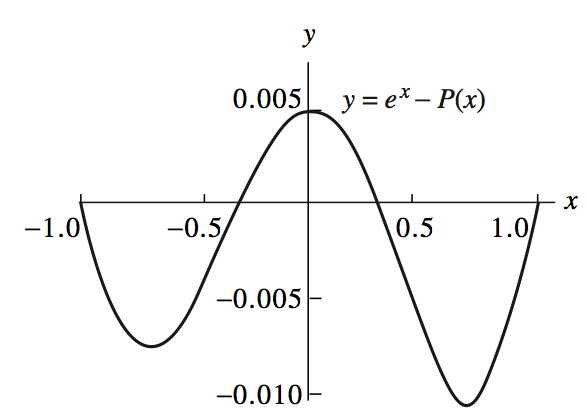
\includegraphics[width=35mm]{chap-3/fig_4-16.png}
\end{center}
\end{figure} 
\end{column}
\begin{column}{0.5\textwidth}
\begin{figure}
\begin{center}
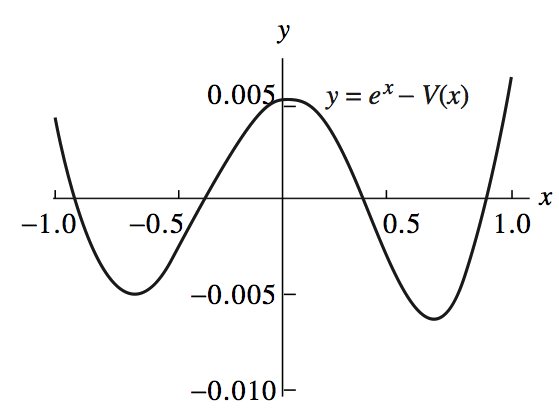
\includegraphics[width=35mm]{chap-3/fig_4-16_2.png}
\end{center}
\end{figure} 
\end{column}
\end{columns}
}

\frame{
\frametitle{Runge Phenomenon}
\begin{itemize}
\item We now look deeper to see the advantage of using the Chebyshev interpolation nodes. 
\item Consider Lagrange interpolating to $f (x)$ over the interval $[-1, 1]$ based on equally spaced nodes. 
\item Does the error $E_N (x) = f(x) - P_N(x)$ tend to zero as $N$ increases? 
\item For functions like $sin(x)$ or $e^x$, where all the derivatives are bounded by the same constant $M$, the answer is yes. 
\item In general, the answer to this question is no, and it is easy to find functions for which the sequence $\{ P_N(x) \}$ does not converge. 
\item If $f(x) = 1 \slash (1 + 12x^2)$, the maximum of the error term $E_N(X)$ grows when $N \rightarrow \infty$. 
\item This nonconvergence is called the {\Large Runge phenomenon}. 
\end{itemize}
}

\frame{
\begin{itemize}
\item The Lagrange polynomial of degree 10 based on 11 equally spaced nodes for this function is shown in Figure 3.17(a). 
\item Wild oscillations occur near the end of the interval. 
\item If the number of nodes is increased, then the oscillations become larger. 
\item This problem occurs because the nodes are equally spaced! 
\end{itemize}
\begin{figure}
\begin{center}
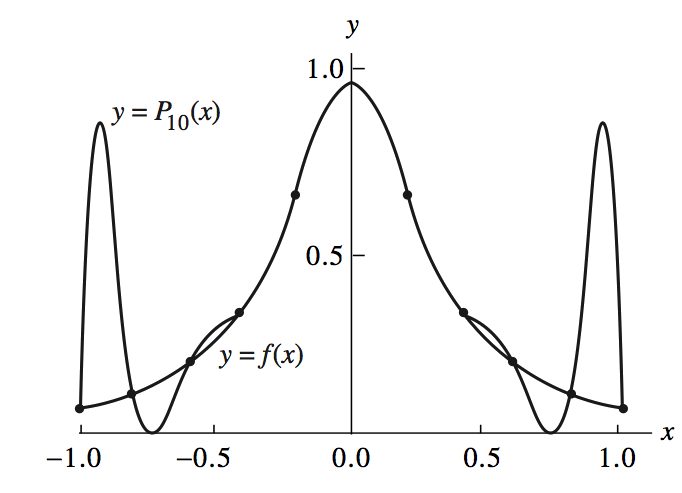
\includegraphics[width=60mm]{chap-3/fig_4-17.png}
\end{center}
\end{figure} 
}


\frame{
\begin{itemize}
\item If the Chebyshev nodes are used to construct an interpolating polynomial of degree $10$ to $f(x) = 1 \slash (1 + 12x^2)$, the error is much smaller, as seen in Figure 3.17(b). 
\item Under the condition that Chebyshev nodes be used, the error $E_N(x)$ will go to zero as $N \to \infty$. 
\item In general, if $f(x)$ and $f'(x)$ are continuous on $[-1,1]$, then it can be proved that Chebyshev interpolation will produce a sequence of polynomials $\{ P_N(x) \}$ that converges uniformly to $f(x)$ over $[-1,1]$. 
\end{itemize}
\begin{figure}
\begin{center}
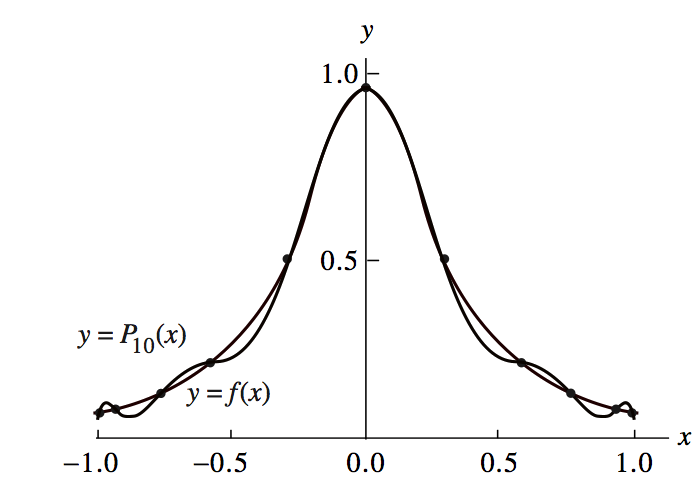
\includegraphics[width=60mm]{chap-3/fig_4-17_2.png}
\end{center}
\end{figure} 
}

\frame{
\frametitle{Transforming the Interval}
Sometimes it is necessary to take a problem stated on an interval $[a, b]$ and reformulate the problem on the interval $[c, d]$ where the solution is known. 
If the approximation $P_N(x)$ to $f(x)$ is to be obtained on the interval $[a, b]$, then we change the variable so that the problem is reformulated on $[-1,1]$: 
\begin{equation*}
x = \left( \frac{b - a}{2} \right) t + \frac{b + a}{2} \ \ \ or \ \ \ t = 2 \frac{x-a}{b-a} - 1
\end{equation*}
where $a \le x \le b$ and $-1 \le t \le 1$. \\
The required Chebyshev nodes of $T_{N+1}(t)$ on $[-1,1]$ are
\begin{equation*}
t_k = \cos	\left( \left( 2N + 1 - 2k\right) \frac{\pi}{2N+2} \right) \ \ \ for \ \ k = 0, 1, \ldots, N
\end{equation*}
and the interpolating nodes on $[a, b]$ are obtained by using (3.88):
\begin{equation*}
x_k = t_k \frac{b-a}{2} + \frac{a+b}{2} \ \ \ for \ \ k = 0, 1, \ldots, N
\end{equation*}
}

\frame{
\begin{block}{Theorem 3.8 (Lagrange-Chebyshev Approximation Polynomial).} 
Assume that $P_N (x)$ is the Lagrange polynomial that is based on the Chebyshev nodes given in equation (3.90).
If $f \in C^{N+1} [a, b]$, then
\begin{equation*}
\left| f (x) - P_N (x) \right| \le \frac{2(b - a)^{N+1}}{ 4^{N+1} (N + 1)!} \max_{a \le x \le b} \left\{ \left| f^{(N+1)}(x) \right|\right\}
\end{equation*}
\end{block}
Example 3.15. \\
For $f (x) = \sin(x)$ on $[0, \pi \slash4]$, find the Chebyshev nodes and the error bound (3.91) for the Lagrange polynomial $P_5(x)$.

Formulas (12), (13), and (14) are used to find the nodes;
\begin{equation*}
x_k = \cos	\left( \frac{(11 - 2k) \pi}{12} \right) \frac{\pi}{8} + \frac{\pi}{8} \ \ \ for \ \ k = 0, 1, \ldots, 5.
\end{equation*}
Using the bound $\left| f^{(6)} (x) \right| \le \left|-\sin( \pi \slash 4) \right| = 2^{-1\slash 2} = M$ in (3.91), 
we get
\begin{equation*}
\left| f (x) - P_N (x) \right| \le  \left( \frac{\pi}{8} \right)^{6}  \left( \frac{2}{6!} \right) 2^{-1 \slash 2} \le 0.00000720
\end{equation*}
}

\frame{
\frametitle{Orthogonal Property}
\framesubtitle{正交特性}
\begin{itemize}
\item In Example 3.14, the Chebyshev nodes were used to find the Lagrange interpolating polynomial. 
\item In general, this implies that the Chebyshev polynomial of degree $N$ can be obtained by Lagrange interpolation based on the $N + 1$ nodes that are the $N + 1$ zeros of $T_{N + 1} (X)$. 
\item However, a direct approach to finding the approximation polynomial is to express $P_N(x)$ as a linear combination of the polynomials $T_k(x)$, which were given in Table 3.11. 
\item Therefore, the Chebyshev interpolating polynomial can be written in the form 
\end{itemize}
\begin{equation*}
P_N (x) = \sum_{k=0}^N c_k T_k (x) = c_0 T_0(x) + c_1 T_1(x) + \cdots + c_N T_N (x).
\end{equation*}
}

\frame{
The coefficients $\{ c_k \}$ in (3.92) are easy to find. 
The technical proof requires the use of the following orthogonality properties. 
Let
\begin{equation*}
x+k = \cos\left( \pi \frac{2k+1}{2N+2} \right) \ \ \  for \ \ k = 0, 1, \ldots, N
\end{equation*}
\begin{equation*}
\sum_{k=0}^N T_i (x_k) T_j (x_k) = 0 \ \ \ when \ \ \ i \neq j
\end{equation*}
\begin{equation*}
\sum_{k=0}^N T_i (x_k) T_j (x_k) = \frac{N+1}{2} \ \ \ when \ \ \ i = j \neq 0
\end{equation*}
\begin{equation*}
\sum_{k=0}^N T_0 (x_k) T_0 (x_k) = N+1
\end{equation*}
Property 4 and the identities (3.94) and (3.96) can be used to prove the following theorem. 
}

\frame{
\begin{block}{Theorem 3.9 (Chebyshev Approximation).} 
The Chebyshev approximation polynomial $P_N (x)$ of degree $ \le N$ for $f (x)$ over $[-1, 1]$ can be written as a sum of $\{ T_j (x) \}$:
\begin{equation*}
f(x) \approx P_N(x) = \sum_{j=0}^N c_j T_j (x)
\end{equation*}
The coefficients $\{ c_j \}$ are computed with the formulas
\begin{equation*}
c_0 = \frac{1}{N+1} \sum_{k=0}^N f(x_k) T_0 (x_k) = \frac{1}{N+1} \sum_{k=0}^N f(x_k)
\end{equation*}
and
\begin{equation*}
\begin{array}{l c l}
c_j & = & \frac{2}{N+1} \sum_{k=0}^N f(x_k) T_j (x_k) \\
& = & \frac{2}{N+1} \sum_{k=0}^N f(x_k) \cos \left( \frac{j \pi (2k+1)}{2N+2} \right)
\end{array}
\end{equation*}
for $j = 1, 2,\ldots, N$
\end{block}
}

\frame{
\frametitle{Example 3.16.} 
Find the Chebyshev polynomial $P_3(x)$ that approximates the function $f (x) = e^x$ over $[-1, 1]$.

The coefficients are calculated using formulas (3.98) and (3.99), and the nodes $x_k = \cos ( \pi (2k + 1) \slash 8)$ for $k = 0, 1, 2, 3$.
\begin{equation*}
\begin{array}{l c l c l}
c_0 & = & \frac{1}{4}\sum_{k=0}^3 e^{x_k} T_0 (x_k) & = & \frac{1}{4}\sum_{k=0}^3 e^{x_k} = 1.26606568 \\
c_1 & = & \frac{1}{2}\sum_{k=0}^3 e^{x_k} T_1 (x_k) & = & \frac{1}{2}\sum_{k=0}^3 e^{x_k} x_k = 1.13031500 \\
c_2 & = & \frac{1}{2}\sum_{k=0}^3 e^{x_k} T_2 (x_k) & = & \frac{1}{2}\sum_{k=0}^3 e^{x_k} \cos \left( 2 \pi \frac{2k+1}{8} \right) = 0.27145036 \\
c_3 & = & \frac{1}{2}\sum_{k=0}^3 e^{x_k} T_3 (x_k) & = & \frac{1}{2}\sum_{k=0}^3 e^{x_k} \cos \left( 3 \pi \frac{2k+1}{8} \right) = 0.04379392
\end{array}
\end{equation*}
Therefore, the Chebyshev polynomial $P_3(x)$ for $e^x$ is
\begin{equation*}
\begin{array}{l c l }
P_3(x) & = & 1.26606568 T_0(x) + 1.13031500 T_1(x) \\
& & + 0.27145036 T_2(x) + 0.04379392 T_3(x).
\end{array}
\end{equation*}
}

\frame{
If the Chebyshev polynomial  is expanded in powers of $x$, the result is
\begin{equation*}
P_3(x) = 0.99461532 + 0.99893324 x + 0.54290072 x^2 + 0.17517568 x^3
\end{equation*}
which is the same as the polynomial $V(x)$ in Example 3.14. 
If the goal is to find the Chebyshev polynomial, formulas (3.98) and (3.99) are preferred
}

